\chapter{Bài toán tìm kiếm}
\section{Giới thiệu}
Bài toán tìm kiếm là một trong những vấn đề thường gặp nhất trong cuộc sống, và kể cả trong máy tính. Tìm một cuốn sách trên tủ sách, tìm chương mà mình yêu thích trong cuốn sách, tìm loại nội dung đang tìm trong đó\dots. Thật vô vàn ví dụ thực tế. Ở đây mình sẽ trình bày những thuật toán tìm kiếm cơ bản trong tìm kiếm dữ liệu trên máy tính.

Đối với các CTDL cây, mình sẽ không trình bày cách thêm, xoá nút cho cây, các bạn tự tìm hiểu nhé.

\section{Tìm kiếm tuần tự}
Phát biểu bài toán: Cho dãy số S. Tìm vị trí giá trị $x$ trong dãy.

Đơn giản là dùng một vòng lặp duy nhất duyệt toàn bộ S, nếu trong quá trình duyệt ta tìm được giá trị $S_i=x$ thì dừng / tìm tiếp tuỳ theo yêu cầu bài toán và thông báo kết quả. Dễ nhận thấy rằng độ phức tạp tính toán trung bình của thuật toán này là $O(n)$. Với n rất lớn, thuật toán này sẽ thất bại.

\section{Tìm kiếm nhị phân}
Bình thường khi tìm một con số trên một dãy số tăng dần / giảm dần, bạn sẽ tìm từ trái sang phải, phải sang trái hay đoán vị trí mà giá trị cần tìm có thể ở đó và chỉ tìm kiếm tại khu vực đó? Thuật toán tìm kiếm nhị phân được xây dựng trên tư tưởng thứ hai, và vì vậy, nó chỉ hoạt động nếu danh sách đã được sắp xếp, nếu không, không còn cách nào khác ngoài tìm kiếm tuần tự như trong thực tế.

Giả sử $S=\{S_1,S_2,\dots,S_n\}$.

Ta sẽ tìm kiếm trên đoạn [l, r] với l = 1, r = n. Thuật toán lặp lại với việc kiểm tra giá trị giữa đoạn. Ta sẽ kiểm tra $S_{n/2}$ có bằng x không:
\begin{itemize}
    \item Nếu $S_{n/2}=x$, trả về giá trị $n/2$. Thuật toán kết thúc.
    \item Nếu $S_{n/2}>x$, vậy x phải nằm ở nửa bên trái của mảng, ta lặp lại thuật toán với nửa mảng con trái bằng cách đặt $r=m-1$.
    \item Nếu $S_{n/2}<x$, tương tự ta đặt $l=m+1$.
\end{itemize}

Cách cài đặt vừa được mô tả ở trên là cách cài đặt tuyến tính dùng một vòng lặp while. Có thể được cài đặt bằng đệ quy, nhưng vì tốc độ của đệ quy chậm hơn vòng lặp nên mình ưu tiên cài đặt theo cách đầu tiên.

Về độ phức tạp, dễ thấy rằng sau mỗi lần lặp độ dài dãy giảm đi 1 nửa, vậy chỉ mất $\log_2n$ thao tác thì độ dài mảng chỉ còn 1, ta chỉ việc kiểm tra xem nó có phải x không. Vậy độ phức tạp thời gian của nó là $O(\log_2n)$.

\section{Cây tìm kiếm nhị phân (Binary Search Tree - BST)}
Bản chất của cây là tìm kiếm nhị phân, tuy nhiên với tìm kiếm nhị phân ta phải sắp xếp dãy số rồi mới áp dụng được, đối với cây tìm kiếm nhị phân trong quá trình ta nhập dãy ta sẽ xây dựng cây luôn, sau đó tìm giá trị thông qua các nhánh của nó.

Cây là một cây nhị phân cân bằng, với mỗi nút, nút con trái chứa giá trị nhỏ hơn nó và nút con phải chứa giá trị lớn hơn nó. Vậy nếu đi theo nhánh trái đến cuối cây ta sẽ gặp giá trị nhỏ nhất và đi theo nhánh phải đến cuôi cây ta sẽ gặp giá trị lớn nhất.

Ví dụ với dãy S = [4, 7, 3, 5, 2, 6, 1]. Ta xây được cây như sau:

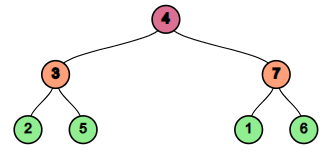
\includegraphics{timkiem/caynpmau.png}

Nguyên tắc xây cây: xây từ trên xuống dưới, từ trái qua phải để đảm bảo tính cân bằng của cây. Dễ nhận thấy nhược điểm rằng thuật toán hoạt động chậm khi cây bị suy biến (cây trở thành một đường thẳng nếu dãy đã được sắp xếp sẵn), lúc này mọi thao tác đều có độ phức tạp tính toán $O(n)$, lúc này người ta sẽ sử dụng cây nhị phân tìm kiếm tối ưu, hoặc dựng cây nhị phân tự cân bằng AVL.

Việc xây cây này cũng là một dạng sắp xếp (người ta gọi phương pháp này là Tree Sort), ta có thể đi theo các nhánh của nó tuỳ vào quan hệ của nó với nút ta đang xét đến khi tìm ra giá trị cần tìm. Và vì chiều cao của cây là $\log_2n$, độ phức tạp \textbf{trung bình} của thuật toán cũng là $O(\log_2n)$. Thời gian xây cây từ một dãy là $O(n)$ và thời gian vừa xây vừa nhập là $O(n\log_2n)$, tương đương với các thuật toán sắp xếp (vì phải đi dọc theo cây để chèn).

\section{Cây tìm kiếm số học (Digital Search Tree - DST)}
Là một cây nhị phân tìm kiếm, nhưng nút con trái của mỗi nút tại mức k của cây sẽ chứa giá trị có bit k là 0, nút con phải sẽ chứa giá trị có bit k là 1. Và vì hiển nhiên giá trị nút con phải lớn hơn cây con trái $2^k$ đơn vị, điều này giống với cây nhị phân tìm kiếm, nhưng lúc này thao tác tìm kiếm trên cây chỉ còn là $O(\log_2\max\{S_i\})$.

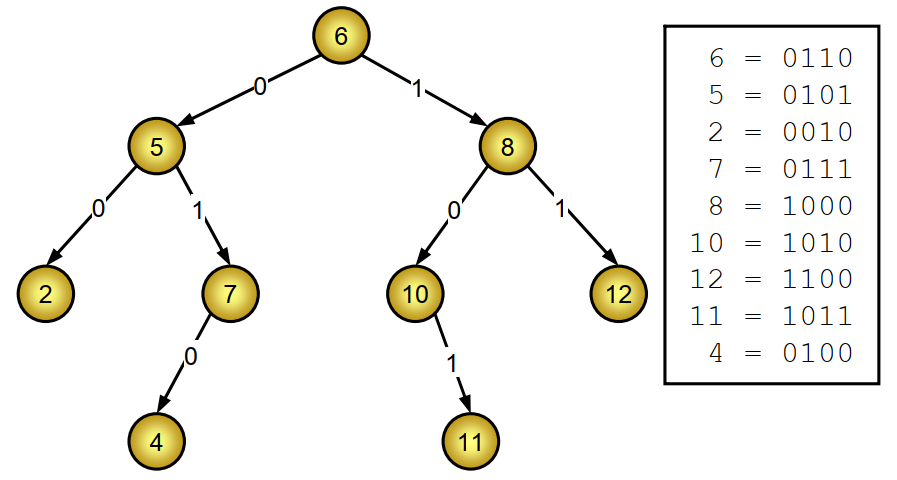
\includegraphics[scale=0.45]{timkiem/caytksohoc.png}

\section{Cây tìm kiếm cơ số (Radix Search Tree - RST)}
Là một cây tìm kiếm số học, nhưng giá trị của dãy chỉ nằm ở các nút lá, còn giá trị trong các nút còn lại là vô nghĩa. Quy ước vẫn giữ nguyên như cây tìm kiếm số học, ta đi theo các nhánh sẽ đến được giá trị cần tìm, nếu không có nút nào ở đó thì tìm kiếm thất bại.

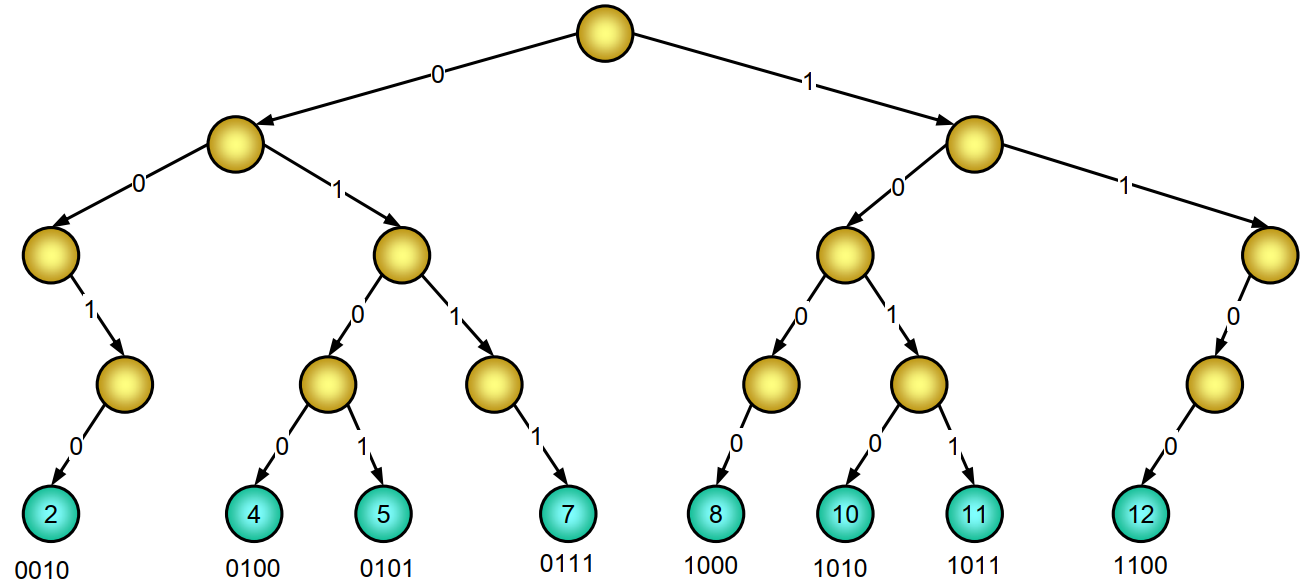
\includegraphics[scale=0.3]{timkiem/caytkcoso2.png}

Các cây tìm kiếm ở trên còn có một nhược điểm: nếu quá trình so sánh giá trị trong khi duyệt phức tạp và mất nhiều thời gian, chúng sẽ hoạt động chậm. RST đã khắc phục được nhược điểm này, nhưng lại có một nhược điểm mới là tốn rất nhiều bộ nhớ vì các giá trị vô nghĩa, ngoài ra để tăng tốc độ tìm kiếm ta có thể dùng cây k-phân thay vì nhị phân nhưng độ phức tạp bộ nhớ sẽ tăng lên.